\documentclass[a4paper,12pt]{report}

\usepackage{cmap}
\usepackage[T2A]{fontenc}
\usepackage[utf8]{inputenc}
\usepackage[english,russian]{babel}
\usepackage{listings}
\usepackage{amsmath}
\usepackage{float}
\usepackage{csquotes}
\usepackage{mathtools}
\usepackage{hyphenat}
\usepackage{amsfonts}
\usepackage{upgreek}

\usepackage{xcolor}
\usepackage{hyperref}

\usepackage{graphicx}
\graphicspath{ {./img/} }

\definecolor{dkgreen}{rgb}{0,0.6,0}
\definecolor{gray}{rgb}{0.5,0.5,0.5}
\definecolor{mauve}{rgb}{0.58,0,0.82}

\lstset{
    language=Python,                 
    basicstyle=\small\sffamily, 
    numbers=left,              
    numberstyle=\tiny,          
    stepnumber=1,                  
    numbersep=5pt,               
    aboveskip=3mm,
    belowskip=3mm,
    showstringspaces=false,
    columns=flexible,
    captionpos=b, 
    basicstyle={\small\ttfamily},
    numbers=left,
    numberstyle=\tiny\color{gray},
    keywordstyle=\color{blue},
    commentstyle=\color{mauve},
    stringstyle=\color{dkgreen},
    breaklines=true,
    breakatwhitespace=true,
    tabsize=3
}

\title{Лабораторная работа №11\\Модуляция и выборка (квантование)}
\author{Смирнов Никита}
\date{\today}

\begin{document}

\maketitle
\tableofcontents
\listoffigures
\lstlistoflistings

\maketitle

\chapter{Упражнение 11.1}

В данном упражнении нам нужно открыть \texttt{chap11.ipynb}, прочитать пояснения и  запустить примеры. Поэтому я просто изучил все примеры с комментариями. 

\chapter{Упражнение 11.2}

В данном упражнении нас просят посмотреть видео \texttt{D/A and A/D | Digital Show and Tell}, 

Это видео о споре качества цифрового и аналогового звука. В нём на примерах объясняется, почему аналоговый звук в допустимых пределах человеческого слуха (от 20 Гц до 20 кГц) может воспроизводиться с идеальной точностью с использованием 16-битного цифрового сигнала 44,1 кГц.

\chapter{Упражнение 11.3}

Для начала загрузим наш звук.

\begin{lstlisting}[caption=Загрузка звука]
wave = thinkdsp.read_wave('2631868.wav')
wave.normalize()
wave.plot()
\end{lstlisting}

\begin{figure}[H]
        \centering
        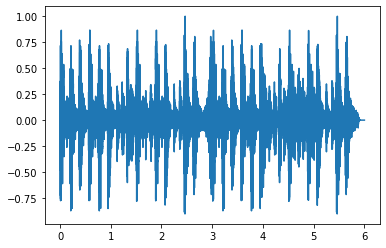
\includegraphics[width=0.75\textwidth]{1.png}
        \caption{Визуализация звука}
        \label{1}
\end{figure}

Этот сигнал дискредитируется с частотой 44100 Гц.

Составим спектр:

\begin{lstlisting}[caption=Спектр звука]
spectrum = wave.make_spectrum(full=True)
spectrum.plot()
\end{lstlisting}

\begin{figure}[H]
        \centering
        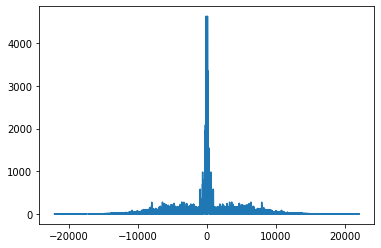
\includegraphics[width=0.75\textwidth]{2.png}
        \caption{Спектр звука}
        \label{2}
\end{figure}

Уменьшим частоту дискретизации в 3 раза:

\begin{lstlisting}[caption=Уменьшение частоты дискретизации]
framerate = wave.framerate / 3
cutoff = framerate / 2 - 1
\end{lstlisting}

Перед дискретизацией мы применяем фильтр сглаживания:

\begin{lstlisting}[caption=Отфильтрованный звук]
spectrum.low_pass(cutoff)
spectrum.plot()
\end{lstlisting}

\begin{figure}[H]
        \centering
        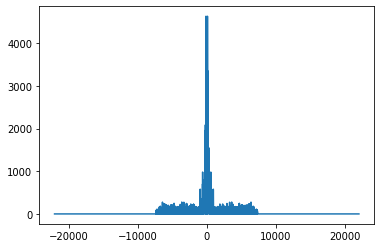
\includegraphics[width=0.75\textwidth]{3.png}
        \caption{Отфильтрованный звук}
        \label{3}
\end{figure}

Следующая функция имитирует процесс выборки:

\begin{lstlisting}[caption=Функция \texttt{sample}]
def sample(wave, factor):
    """Simulates sampling of a wave.
    
    wave: Wave object
    factor: ratio of the new framerate to the original
    """
    ys = np.zeros(len(wave))
    ys[::factor] = wave.ys[::factor]
    return thinkdsp.Wave(ys, framerate=wave.framerate)
\end{lstlisting}

Результат содержит копии спектра около 20 кГц.

\begin{lstlisting}[caption=Спектр звука]
sampled_spectrum = sampled.make_spectrum(full=True)
sampled_spectrum.plot()
\end{lstlisting}

\begin{figure}[H]
        \centering
        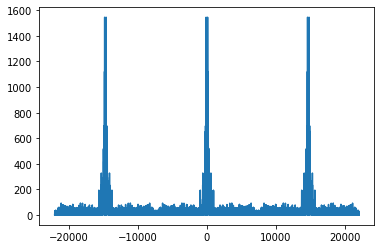
\includegraphics[width=0.75\textwidth]{4.png}
        \caption{Спектр звука}
        \label{4}
\end{figure}

Применяем фильтр сглаживания:

\begin{lstlisting}[caption=Применение фильтра сглаживания]
sampled_spectrum.low_pass(cutoff)
sampled_spectrum.plot()
\end{lstlisting}

\begin{figure}[H]
        \centering
        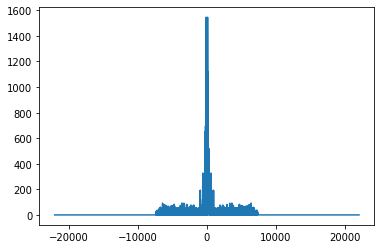
\includegraphics[width=0.75\textwidth]{5.png}
        \caption{Применение фильтра сглаживания}
        \label{5}
\end{figure}

Мы только что потеряли половину энергии в спектре, но мы можем масштабировать результат, чтобы вернуть его:

\begin{lstlisting}[caption=Масштабирование результата]
sampled_spectrum.scale(factor)
spectrum.plot()
sampled_spectrum.plot()
\end{lstlisting}

\begin{figure}[H]
        \centering
        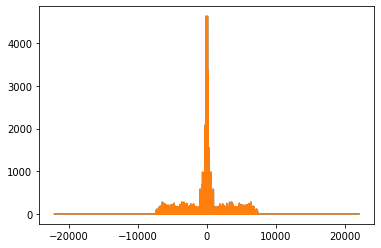
\includegraphics[width=0.75\textwidth]{6.png}
        \caption{Масштабирование результата}
        \label{6}
\end{figure}

Теперь разница между спектром до и после дискретизации должна быть небольшой.

\begin{lstlisting}[caption=Разница между спектром до и после дискретизации]
spectrum.max_diff(sampled_spectrum)
\end{lstlisting}

Разница составила \texttt{1.8189894035458565e-12}.

\begin{lstlisting}[caption=Разница между интерполированной волной и фильтрованной волной]
filtered.plot()
interpolated.plot()
\end{lstlisting}

\begin{figure}[H]
        \centering
        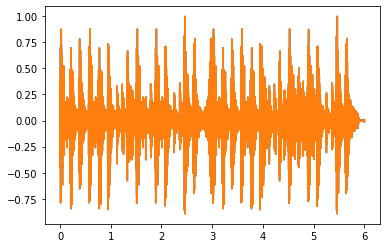
\includegraphics[width=0.75\textwidth]{7.png}
        \caption{Разница между интерполированной волной и фильтрованной волной}
        \label{7}
\end{figure}

\begin{lstlisting}[caption=Разница между интерполированной волной и фильтрованной волной]
filtered.max_diff(interpolated)
\end{lstlisting}

Разница составила \texttt{5.56290642113787e-16}.

Умножение на импульсы даёт 4 сдвинутых копии исходного спектра. Один из них проходит от отрицательного конца спектра к положительному, поэтому в спектре от выбранной волны есть 5 пиков.

\chapter{Выводы}

Во время выполнения лабораторной работы получены навыки работы с эффектом выборки и представил теорему выборки, которая объясняет сглаживание и частоту сворачивания. Также научился применять эти знания на практике.

\end{document}